\begin{name}
	{\tenchude}{\tendethi}{LỚP TOÁN THẦY PHÁT}{\thoigian}
\end{name}
\Opensolutionfile{ans}[ans/ans-2-TT-4-SoBacGiang-23-L1]
\setcounter{ex}{0}\setcounter{bt}{0}

%%%%%%%%%%%%Câu 1
\begin{ex}%[Thi Thử L1, Sở Bắc Giang, 2023]%[Thành Đức Trung, dự án 12-EX-6]%[2D1Y5-1]
\immini{Đồ thị của hàm số nào dưới đây có dạng như đường cong trong hình vẽ bên?
\choice
{$y=\dfrac{x+1}{x-2}$}
{\True $y=x^4-2x^2-3$}
{$y=x^3-3x-3$}
{$y=-x^4+2x^2-3$}
}
{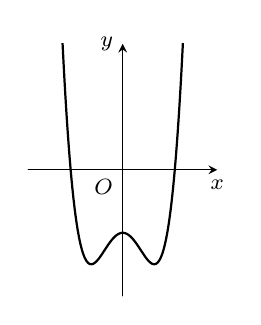
\begin{tikzpicture}[scale=0.4, font=\footnotesize, line join=round, line cap=round, >=stealth]
\def\a{1}
\def\b{-2}
\def\c{-2}
\draw[->] (-3,0) -- (3,0) node[below] {$x$};
\draw[->] (0,-4) -- (0,4) node[left] {$y$};
\draw (0,0)node[below left]{$O$};
\clip (-3,-4)rectangle(3,4);
\draw[thick,samples=150,smooth,domain=-4:4] plot(\x,{\a*(\x)^4+(\b)*(\x)^2+(\c)});
\end{tikzpicture}
}
\loigiai
{Dựa vào hình vẽ đã cho ta thấy đồ thị có dạng đồ thị hàm trùng phương $y=ax^4+bx^2+c$ với $a>0$.\\
Do đó đồ thị hàm số đã cho là đồ thị hàm số $y=x^4-2x^2-3$.
}
\end{ex}

%%%%%%%%%%%%Câu 2
\begin{ex}%[Thi Thử L1, Sở Bắc Giang, 2023]%[Thành Đức Trung, dự án 12-EX-6]%[1D2Y2-1]
Cho đa giác đều có 20 đỉnh. Số tam giác được tạo thành có các đỉnh đều là đỉnh của đa giác đã cho là
\choice
{\True $\mathrm{C}_{20}^3$}
{$\mathrm{A}_{20}^3$}
{$\mathrm{P}_3$}
{$\mathrm{P}_20$}
\loigiai
{Số tam giác có các đỉnh đều là đỉnh của đa giác đều 20 cạnh là $\mathrm{C}_{20}^3$.
}
\end{ex}

%%%%%%%%%%%%Câu 3
\begin{ex}%[Thi Thử L1, Sở Bắc Giang, 2023]%[Thành Đức Trung, dự án 12-EX-6]%[2D1Y2-2]
\immini{
Cho hàm số trùng phương $y=f(x)$ có đồ thị là đường cong trong hình bên.
Giá trị cực đại của hàm số đã cho là
\choice
{$-1$}
{$0$}
{$-4$}
{\True $-3$}
}
{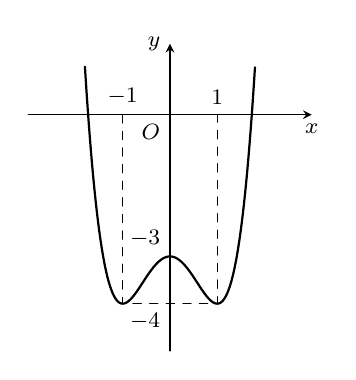
\begin{tikzpicture}[scale=0.6, font=\footnotesize, line join=round, line cap=round, >=stealth]
\def\a{1}
\def\b{-2}
\def\c{-3}
\draw[->] (-3,0) -- (3,0) node[below] {$x$};
\draw[->] (0,-5) -- (0,1.5) node[left] {$y$};
\draw (0,0)node[below left]{$O$};
\clip (-3,-5)rectangle(3,1.5);
\draw[dashed] (-1,0)--(-1,-4)--(1,-4)--(1,0);
\draw (-1,0) node[above]{$-1$};
\draw (1,0) node[above]{$1$};
\draw (0,-3) node[above left]{$-3$};
\draw (0,-4) node[below left]{$-4$};
\draw[thick,samples=150,smooth,domain=-1.8:1.8] plot(\x,{\a*(\x)^4+(\b)*(\x)^2+(\c)});
\end{tikzpicture}
}
\loigiai
{Dựa vào hình vẽ ta thấy giá trị cực đại của hàm số là $-3$.
}
\end{ex}

%%%%%%%%%%%%Câu 7
\begin{ex}%[Thi Thử L1, Sở Bắc Giang, 2023]%[Thành Đức Trung, dự án 12-EX-6]%[2H1Y3-2]
Cho khối lập phương có cạnh bằng $3\,\text{cm}$. Thể tích của khối lập phương đã cho bằng
\choice
{\True $27\,\text{cm}^3$}
{$\dfrac{27}{2}\,\text{cm}^3$}
{$9\,\text{cm}^3$}
{$18\,\text{cm}^3$}
\loigiai
{Thể tích của khối lập phương cạnh bằng $3$ là $V=3^3=27\,\text{cm}^3$.
}
\end{ex}

%%%%%%%%%%%%Câu 8
\begin{ex}%[Thi Thử L1, Sở Bắc Giang, 2023]%[Thành Đức Trung, dự án 12-EX-6]%[2D3Y1-1]
Cho $\displaystyle\int\cos x\mathrm{\,d}x=F(x)+C$. Khẳng định nào dưới đây đúng?
\choice
{$F'(x)=-\sin x$}
{$F'(x)=\sin x$}
{$F'(x)=-\cos x$}
{\True $F'(x)=\cos x$}
\loigiai
{Theo định nghĩa nguyên hàm, ta có $\displaystyle\int\cos x\mathrm{\,d}x=F(x)+C\Rightarrow F'(x)=\cos x$.
}
\end{ex}

%%%%%%%%%%%%Câu 9
\begin{ex}%[Thi Thử L1, Sở Bắc Giang, 2023]%[Thành Đức Trung, dự án 12-EX-6]%[2H3Y2-2]
Trong KG $Oxyz$, mặt phẳng $(P)\colon x-y+z+1=0$ có một véc-tơ pháp tuyến là
\choice
{$\overrightarrow{n}_4=(1;1;-1)$}
{$\overrightarrow{n}_3=(1;1;1)$}
{\True $\overrightarrow{n}_2=(1;-1;1)$}
{$\overrightarrow{n}_1=(-1;1;1)$}
\loigiai
{Mặt phẳng $(P)\colon x-y+z+1=0$ có một véc-tơ pháp tuyến là $\overrightarrow{n}_2=(1;-1;1)$.
}
\end{ex}

%%%%%%%%%%%%Câu 11
\begin{ex}%[Thi Thử L1, Sở Bắc Giang, 2023]%[Thành Đức Trung, dự án 12-EX-6]%[2D4Y2-2]
Cho số phức $z=2+i$, phần thực của số phức $z^2$ bằng
\choice
{$-4$}
{$4$}
{\True $3$}
{$-3$}
\loigiai
{Ta có 
\[z^2=(2+i)^2=2^2+2\cdot 2\cdot i+i^2=4+4i-1=3+4i.\]
Vậy phần thực của số phức $z^2$ là 3.
}
\end{ex}

%%%%%%%%%%%%Câu 13
\begin{ex}%[Thi Thử L1, Sở Bắc Giang, 2023]%[Thành Đức Trung, dự án 12-EX-6]%[2D3Y2-1]
Nếu $\displaystyle\int\limits_2^5 f(x)\mathrm{\,d}x=3$ và $\displaystyle\int\limits_2^5 g(x)\mathrm{\,d}x=-2$ thì $\displaystyle\int\limits_2^5 [f(x)-g(x)]\mathrm{\,d}x$ bằng
\choice
{$-5$}
{$-6$}
{$1$}
{\True $5$}
\loigiai
{Ta có \[\displaystyle\int\limits_2^5 [f(x)-g(x)]\mathrm{\,d}x=\displaystyle\int\limits_2^5 f(x)\mathrm{\,d}x-\displaystyle\int\limits_2^5 g(x)\mathrm{\,d}x=3-(-2)=5.\]
}
\end{ex}

%%%%%%%%%%%%Câu 14
\begin{ex}%[Thi Thử L1, Sở Bắc Giang, 2023]%[Thành Đức Trung, dự án 12-EX-6]%[1D3Y4-3]
Cho cấp số nhân $(u_n)$ với $u_1=3$ và công bội $q=\dfrac{1}{3}$. Giá trị của $u_3$ bằng
\choice
{$1 $}
{$\dfrac{4}{3}$}
{$\dfrac{1}{9}$}
{\True $\dfrac{1}{3}$}
\loigiai
{Ta có $u_3=u_1\cdot q^2=3\cdot \left(\dfrac{1}{3}\right)^2=\dfrac{1}{3}$.
}
\end{ex}

%%%%%%%%%%%%Câu 15
\begin{ex}%[Thi Thử L1, Sở Bắc Giang, 2023]%[Thành Đức Trung, dự án 12-EX-6]%[2D2Y6-1]
Tập nghiệm của bất phương trình $\left(\dfrac{1}{3}\right)^x\ge 9$ là
\choice
{$(-\infty;2)$}
{\True $(-\infty;-2]$}
{$[-2;+\infty)$}
{$(-\infty;-2)$}
\loigiai
{Ta có $\left(\dfrac{1}{3}\right)^x\ge 9\Leftrightarrow \left(\dfrac{1}{3}\right)^x\ge \left(\dfrac{1}{3}\right)^{-2}\Leftrightarrow x\le -2$.\\
Vậy tập nghiệm của bất phương trình đã cho là $S=(-\infty;-2]$.
}
\end{ex}

%%%%%%%%%%%%Câu 19
\begin{ex}%[Thi Thử L1, Sở Bắc Giang, 2023]%[Thành Đức Trung, dự án 12-EX-6]%[2H2Y1-2]
Cho hình trụ có bán kính đáy $r$ và chiều cao $h$. Diện tích toàn phần của hình trụ đã cho bằng
\choice
{\True $2\pi r(r+h)$}
{$\pi rh$}
{$2\pi rh$}
{$\pi r(r+h)$}
\loigiai
{Diện tích toàn phần của hình trụ có bán kính đáy $ r $ và chiều cao $ h $ bằng 
\[S_{\text{tp}}=S_{\text{xq}}+2\cdot S_{\text{đáy}}=2\pi rh+2\cdot\pi r^2=2\pi r(r+h).\]
}
\end{ex}

%%%%%%%%%%%%Câu 20
\begin{ex}%[Thi Thử L1, Sở Bắc Giang, 2023]%[Thành Đức Trung, dự án 12-EX-6]%[2D1Y5-4]
\immini{
Cho hàm số $y=\dfrac{ax+b}{cx+d}$ có đồ thị là đường cong trong hình vẽ bên. 
Tọa độ giao điểm của đồ thị hàm số đã cho và trục tung là
\choice
{$(0;2)$}
{$(-2;0)$}
{$(2;0)$}
{\True $(0;-2)$}
}
{
\begin{tikzpicture}[scale=0.5, font=\footnotesize, line join=round, line cap=round, >=stealth]
\def\a{1}
\def\b{-2}
\def\c{1}
\def\d{1}
\draw[->] (-6,0) -- (5,0) node[below] {$x$};
\draw[->] (0,-5) -- (0,5) node[left] {$y$};
\draw (0,0)node[below left]{$O$};
\draw[dashed,blue] (-1,-5)--(-1,5) (-6,1)--(5,1); % Vẽ TCĐ và TCN
\clip (-6,-5)rectangle(5,5);
\pgfmathsetmacro{\can}{-(\d)/(\c)}
\draw[thick,samples=150,smooth,domain=-6:{\can-.1}] plot(\x,{(\a*\x+(\b))/(\c*\x+(\d))});
\draw[thick,samples=150,smooth,domain={\can+.1}:5] plot(\x,{(\a*\x+(\b))/(\c*\x+(\d))});
\draw (2,0) node[below]{$2$};
\draw (0,-2) node[right]{$-2$};
\draw (-1,0) node[below left]{$-1$};
\draw (0,1) node[above right]{$1$};
\end{tikzpicture}
}
\loigiai
{Dựa vào hình vẽ ta thấy đồ thị hàm số đã cho cắt trục tung tại điểm $(0;-2)$.
}
\end{ex}

%%%%%%%%%%%%Câu 21
\begin{ex}%[Thi Thử L1, Sở Bắc Giang, 2023]%[Thành Đức Trung, dự án 12-EX-6]%[2D4Y1-1]
Phần ảo của số phức $z=-4+3i$ là
\choice
{$-4$}
{$4$}
{$3i$}
{\True $3$}
\loigiai
{Phần ảo của số phức $z=-4+3i$ là $3$.
}
\end{ex}

%%%%%%%%%%%%Câu 22
\begin{ex}%[Thi Thử L1, Sở Bắc Giang, 2023]%[Thành Đức Trung, dự án 12-EX-6]%[2D4Y1-2]
Trong mặt phẳng tọa độ $Oxy$, điểm biểu diễn của số phức $z=2-3i$ có tọa độ là
\choice
{$(3;2)$}
{\True $(2;-3)$}
{$(-3;2)$}
{$(2;3)$}
\loigiai
{Điểm biểu diễn của số phức $z=2-3i$ có tọa độ là $(2;-3)$.
}
\end{ex}

%%%%%%%%%%%%Câu 23
\begin{ex}%[Thi Thử L1, Sở Bắc Giang, 2023]%[Thành Đức Trung, dự án 12-EX-6]%[2D2Y4-2]
Trên khoảng $(0;+\infty)$, đạo hàm của hàm số $y=\log_2 x$ là
\choice
{$y'=x\ln 2$}
{$y'=\dfrac{x}{\ln 2}$}
{\True $y'=\dfrac{1}{x\ln 2}$}
{$y'=\dfrac{\ln 2}{x}$}
\loigiai
{Ta có $y=\log_2 x$ suy ra $y'=\dfrac{1}{x\ln 2}$.
}
\end{ex}

%%%%%%%%%%%%Câu 24
\begin{ex}%[Thi Thử L1, Sở Bắc Giang, 2023]%[Thành Đức Trung, dự án 12-EX-6]%[2D1Y1-2]
Cho hàm số $y=f(x)$ có bảng biến thiên như sau:
\begin{center}

\begin{tikzpicture}
\tkzTab[nocadre=false,lgt=1.2,espcl=2.5,deltacl=0.6]
{$x$/1, $y'$/1, $y$/2.5}
{$-\infty$, $0$, $3$, $+\infty$}
{,-,0,+,0,-,}
{+/ $+\infty$, -/ $-4$, +/ $-1$ , -/ $-\infty$}
\end{tikzpicture}
\end{center}
Hàm số đã cho đồng biến trên khoảng nào dưới đây?
\choice
{$(-\infty;1)$}
{$(3;+\infty)$}
{$(-4;-1)$}
{\True $(0;3)$}
\loigiai
{Dựa vào bảng biến thiên ta thấy hàm số đã cho đồng biến trên $(0;3)$.
}
\end{ex}

%%%%%%%%%%%%Câu 26
\begin{ex}%[Thi Thử L1, Sở Bắc Giang, 2023]%[Thành Đức Trung, dự án 12-EX-6]%[2H3Y1-3]
Trong không gian với hệ tọa độ $O x y z$, tâm của mặt cầu $(S)\colon x^2+y^2+z^2+2 x-4 y+6 z-1=0$ có toạ độ là
\choice
{$(-2 ; 4 ;-6)$}
{$(1 ;-2 ; 3)$}
{\True $(-1 ; 2 ;-3)$}
{$(2 ;-4 ; 6)$}
\loigiai
{
Tâm của mặt cầu $(S)\colon x^2+y^2+z^2+2 x-4 y+6 z-1=0$ có toạ độ là $I(-1;2;-3)$.
}
\end{ex}

%%%%%%%%%%%%Câu 27
\begin{ex}%[Thi Thử L1, Sở Bắc Giang, 2023]%[Thành Đức Trung, dự án 12-EX-6]%[2D1Y5-3]
\immini{
Cho hàm số bậc ba $y=f(x)$ có đồ thị là đường cong trong hình bên. Có tất cả bao nhiêu giá trị nguyên dương của tham số $m$ để phương trình $f(x)-1=m$ có đúng ba nghiệm thực phân biệt?
\choice
{\True $3$}
{$4$}
{$1$}
{$2$}
}{
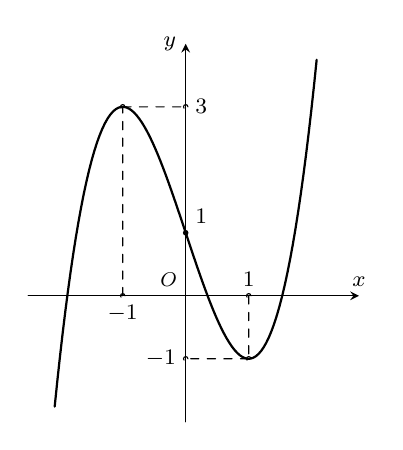
\begin{tikzpicture}[scale = 0.8, font=\footnotesize, line join=round, line cap=round, >=stealth]
\draw[->] (-2.5,0) -- (0,0) node[above left, scale = 0.9]{$O$} -- (2.75,0) node[above]{$x$};
\draw[->] (0,-2) -- (0,4) node[left]{$ y $};
\tkzDrawPoint[fill = black](0,0);
\draw[color = black, thick] plot[domain=-2.08:2.08, samples=100](\x,{(\x)^(3.0)-3.0*(\x)+1});
\draw [dashed] (-1,0) circle (1pt) node[below]{$ -1 $} -- (-1,3) circle (1pt) -- (0,3) circle (1pt) node[right]{$ 3 $};
\draw [dashed] (1,0) circle (1pt) node[above]{$ 1 $} -- (1,-1) circle (1pt) -- (0,-1) circle (1pt) node[left]{$ -1 $};
\draw[fill=black] (0,1) circle (1pt) node[above right]{$1$};
\end{tikzpicture}
}
\loigiai
{
Để phương trình $f(x)-1=m \Leftrightarrow f(x) = m+1$ có đúng ba nghiệm thực phân biệt thì $-1<m+1< 3\Leftrightarrow -2<m<2$.\\
Vậy có $3$ giá trị nguyên của tham số $m$ là $\left\{-1;0;1\right\}$ thỏa mãn đề bài.
}
\end{ex}

%%%%%%%%%%%%Câu 28
\begin{ex}%[Thi Thử L1, Sở Bắc Giang, 2023]%[Thành Đức Trung, dự án 12-EX-6]%[2D2Y3-1]
Với $a$ là số thực dương tùy ý khác $4$, giá trị của biểu thức $\log _{\frac{a}{4}}\left(\dfrac{a^3}{64}\right)$ bằng
\choice
{$\dfrac{1}{3}$}
{$-3$}
{$-\dfrac{1}{3}$}
{\True $3$}
\loigiai
{
Ta có $\log _{\frac{a}{4}}\left(\dfrac{a^3}{64}\right) = \log_{\frac{a}{4}}\left(\dfrac{a}{4}\right)^3 = 3$.
}
\end{ex}

%%%%%%%%%%%%Câu 29
\begin{ex}%[Thi Thử L1, Sở Bắc Giang, 2023]%[Thành Đức Trung, dự án 12-EX-6]%[2D1Y4-1]
Tiệm cận đứng của đồ thị hàm số $y=\dfrac{2 x+3}{4 x+2}$ là đường thẳng có phương trình
\choice
{$x=\dfrac{3}{2}$}
{$x=-\dfrac{3}{2}$}
{\True $x=-\dfrac{1}{2}$}
{$x=\dfrac{1}{2}$}
\loigiai
{
Tiệm cận đứng của đồ thị hàm số $y=\dfrac{2 x+3}{4 x+2}$ là đường thẳng có phương trình $x = -\dfrac{1}{2}$.
}
\end{ex}

%%%%%%%%%%%%Câu 30
\begin{ex}%[Thi Thử L1, Sở Bắc Giang, 2023]%[Thành Đức Trung, dự án 12-EX-6]%[2D2Y2-2]
Trên khoảng $(0 ;+\infty)$, đạo hàm của hàm số $y=x^{2 \pi}$ là
\choice
{$y'=\dfrac{1}{2 \pi} x^{2 \pi-1}$}
{\True $y'=2 \pi x^{2 \pi-1}$}
{$y'=2 \pi x^{2 \pi}$}
{$y'=x^{2 \pi-1}$}
\loigiai
{ Ta có $y' = 2\pi\cdot x^{2\pi -1}$.
}
\end{ex}

%%%%%%%%%%%%Câu 31
\begin{ex}%[Thi Thử L1, Sở Bắc Giang, 2023]%[Thành Đức Trung, dự án 12-EX-6]%[2H3Y2-5]
Trong KG $Oxyz$, góc giữa hai mặt phẳng $(O x z)$ và $(O y z)$ bằng
\choice
{\True $90^{\circ}$}
{$60^{\circ}$}
{$30^{\circ}$}
{$45^{\circ}$}
\loigiai
{
Góc giữa hai mặt phẳng $(O x z)$ và $(O y z)$ bằng $90^\circ$.
}
\end{ex}

%%%%%%%%%%%%Câu 32
\begin{ex}%[Thi Thử L1, Sở Bắc Giang, 2023]%[Thành Đức Trung, dự án 12-EX-6]%[2D3Y1-1]
Cho hàm số $f(x)=\mathrm{e}^x-\sin x$. Khẳng định nào dưới đây đúng?
\choice
{\True $\displaystyle\int f(x) \;\mathrm{d} x=\mathrm{e}^x+\cos x+C$}
{$\displaystyle\int f(x) \;\mathrm{d} x=x \cdot e^{x-1}-\cos x+C$}
{$\displaystyle\int f(x) \;\mathrm{d} x=\frac{\mathrm{e}^{x+1}}{x+1}+\cos x+C$}
{$\displaystyle\int f(x) \;\mathrm{d} x=\mathrm{e}^x-\cos x+C$}
\loigiai
{
Ta có $\displaystyle\int f(x) \;\mathrm{d} x=\mathrm{e}^x+\cos x+C$.
}
\end{ex}

%%%%%%%%%%%%Câu 33
\begin{ex}%[Thi Thử L1, Sở Bắc Giang, 2023]%[Thành Đức Trung, dự án 12-EX-6]%[2H2Y2-1]
Cho mặt phẳng $(P)$ không có điểm chung với mặt cầu $S(O ; R)$. Gọi $d$ là khoảng cách từ $O$ đến $(P)$. Khẳng định nào dưới đây đúng?
\choice
{$d=R$}
{$d<R$}
{\True $d>R$}
{$d=0$}
\loigiai
{ Vì mặt phẳng $(P)$ không có điểm chung với mặt cầu $S(O ; R)$ nên $d > R$.
}
\end{ex}

%%%%%%%%%%%%Câu 34
\begin{ex}%[Thi Thử L1, Sở Bắc Giang, 2023]%[Thành Đức Trung, dự án 12-EX-6]%[2D1Y2-2]
\immini{
Cho hàm số $y=a x^3+b x^2+c x+d$ có đồ thị là đường cong trong hình bên. Điểm cực đại của đồ thị hàm số đã cho có tọa độ là
\choice
{$(1 ;-3)$}
{\True $(1 ; 1)$}
{$(-1 ;-3)$}
{$(0 ;-1)$}
}{
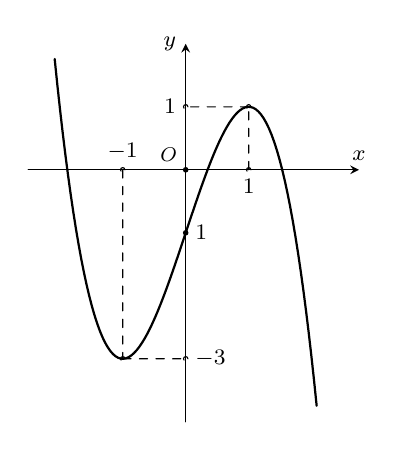
\begin{tikzpicture}[scale = 0.8, font=\footnotesize, line join=round, line cap=round, >=stealth]
\draw[->] (-2.5,0) -- (0,0) node[above left, scale = 0.9]{$O$} -- (2.75,0) node[above]{$x$};
\draw[->] (0,-4) -- (0,2) node[left]{$ y $};
\draw[color = black, thick] plot[domain=-2.08:2.08, samples=100](\x,{-(\x)^(3)+3*(\x)-1});
\draw [dashed] (1,0) circle (1pt) node[below]{$ 1 $} -- (1,1) circle (1pt) -- (0,1) circle (1pt) node[left]{$ 1 $};
\draw [dashed] (-1,0) circle (1pt) node[above]{$ -1 $} -- (-1,-3) circle (1pt) -- (0,-3) circle (1pt) node[right]{$ -3 $};
\draw[fill=black] (0,-1) circle (1pt) node[right]{$1$} (0,0) circle (1pt);
\end{tikzpicture}
}
\loigiai
{
Điểm cực đại của đồ thị hàm số có tọa độ là $\left(1;1\right)$.
}
\end{ex}

%%%%%%%%%%%%Câu 35
\begin{ex}%[Thi Thử L1, Sở Bắc Giang, 2023]%[Thành Đức Trung, dự án 12-EX-6]%[2H2Y2-4]
Trong không gian với hệ tọa độ $O x y z$, cho mặt phẳng $(P)\colon 2 x+3 y-z+3=0$. Điểm nào dưới đây thuôc $(P)$?
\choice
{$E(1 ;-2 ; 0)$}
{$F(-1 ; 2 ;-1)$}
{$M(2 ; 1 ; 3)$}
{\True $N(0 ;-1 ; 0)$}
\loigiai
{
Thay tọa độ từng điểm vào phương trình mặt phẳng $\left(P\right)$, ta có $N(0 ;-1 ; 0)\in\left(P\right)$.
}
\end{ex}

%%%%%%%%%%%%Câu 40
\begin{ex}%[Thi Thử L1, Sở Bắc Giang, 2023]%[Thành Đức Trung, dự án 12-EX-6]%[2H3Y1-1]
Trong không gian với hệ tọa độ $O x y z$, cho điểm $A(2 ;-3 ; 5)$. Tìm tọa độ $A'$ là điểm đối xứng với $A$ qua trục $O y$.
\choice
{$A'(-2 ;-3 ; 5)$}
{$A'(2 ;-3 ;-5)$}
{$A'(2 ; 3 ; 5)$}
{\True $A'(-2 ;-3 ;-5)$}
\loigiai
{
Tọa độ $A'$ là điểm đối xứng với $A$ qua trục $O y$ là $\left(-2;-3;-5\right)$.
}
\end{ex}

%%%%%%%%%%%%Câu 4
\begin{ex}%[Thi Thử L1, Sở Bắc Giang, 2023]%[Thành Đức Trung, dự án 12-EX-6]%[2D2B5-3]
Tổng tất cả các nghiệm thực của phương trình $4^x-3\cdot 2^{x+2}+32=0$ bằng
\choice
{$6$}
{\True $5$}
{$-6$}
{$-5$}
\loigiai
{Ta có
\[4^x-3\cdot 2^{x+2}+32=0\Leftrightarrow (2^x)^2-12\cdot 2^x+32=0\Leftrightarrow\hoac{&2^x=4\\&2^x=8}\Leftrightarrow \hoac{&2^x=2^2\\&2^x=2^3}\Leftrightarrow\hoac{&x=2\\&x=3.}\]
Tổng các nghiệm của phương trình đã cho bằng $2+3=5$.
}
\end{ex}

%%%%%%%%%%%%Câu 5
\begin{ex}%[Thi Thử L1, Sở Bắc Giang, 2023]%[Thành Đức Trung, dự án 12-EX-6]%[2D3B2-1]
Nếu $\displaystyle\int\limits_0^1 2f(x)\mathrm{\,d}x=6$ thì $\displaystyle\int\limits_0^1\left[\dfrac{1}{3}f(x)+2x\right]\mathrm{\,d}x$ bằng
\choice
{$4$}
{$7$}
{$3$}
{\True $2$}
\loigiai
{Ta có
\[\displaystyle\int\limits_0^1\left[\dfrac{1}{3}f(x)+2x\right]\mathrm{\,d}x=\dfrac{1}{6}\displaystyle\int\limits_0^1 2f(x)\mathrm{\,d}x+\displaystyle\int\limits_0^1 2x\mathrm{\,d}x=\dfrac{1}{6}\cdot 6+x^2\Big|_0^1=1+1^2-0^2=2.\]
}
\end{ex}

%%%%%%%%%%%%Câu 6
\begin{ex}%[Thi Thử L1, Sở Bắc Giang, 2023]%[Thành Đức Trung, dự án 12-EX-6]%[2H1B3-2]
Cho hình chóp $S.ABC$ có đáy $ABC$ là tam giác đều với $AB=a$, $SA\perp(ABC)$ và $SA=a\sqrt{3}$. Thể tích khối chóp $S.ABC$ bằng
\choice
{$a^3$}
{$\dfrac{a^3\sqrt{3}}{4}$}
{$\dfrac{3a^2}{4}$}
{\True $\dfrac{a^3}{4}$}
\loigiai
{\immini
{Do tam giác $ABC$ đều cạnh $a$ nên diện tích tam giác $ABC$ là $S_{\triangle ABC}=\dfrac{a^2\sqrt{3}}{4}$.\\
Thể tích khối chóp $S.ABC$ là $V=\dfrac{1}{3}\cdot SA\cdot S_{\triangle ABC}=\dfrac{1}{3}\cdot a\sqrt{3}\cdot\dfrac{a^2\sqrt{3}}{4}=\dfrac{a^3}{4}$.
}
{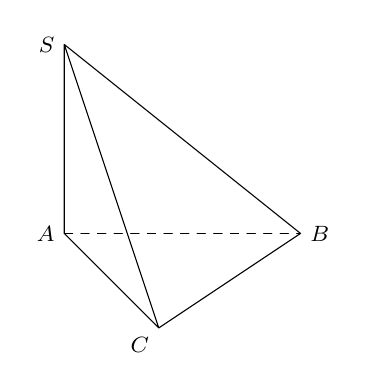
\begin{tikzpicture}[scale=0.6, font=\footnotesize, line join=round, line cap=round, >=stealth]
\draw (0,4)--(0,0)--(2,-2)--(5,0)--(0,4)--(2,-2);
\draw[dashed] (0,0)--(5,0);
\draw (0,4) node[left]{$S$};
\draw (0,0) node[left]{$A$};
\draw (5,0) node[right]{$B$};
\draw (2,-2) node[below left]{$C$};
\end{tikzpicture}
}
}
\end{ex}

%%%%%%%%%%%%Câu 10
\begin{ex}%[Thi Thử L1, Sở Bắc Giang, 2023]%[Thành Đức Trung, dự án 12-EX-6]%[2D4B3-4]
Cho số phức $z$ thỏa mãn $|z-1+2i|=3$. Biết tập hợp các điểm biểu diễn số phức $w=z(1+i)$ trong mặt phẳng tọa độ là một đường tròn. Tìm bán kính $R$ của đường tròn đó.
\choice
{\True $R=3\sqrt{2}$}
{$R=4\sqrt{2}$}
{$R=\sqrt{2}$}
{$R=2\sqrt{2}$}
\loigiai
{Ta có 
\[w=z(1+i)\Leftrightarrow w=(z-1+2i)(1+i)+3-i\Leftrightarrow w-3+i=(z-1+2i)(1+i).\]
Lấy mô-đun 2 vế ta được
\[|w-3+i|=|z-1+2i|\cdot |1+i|=3\sqrt{2}.\]
Vậy tập hợp các điểm biểu diễn số phức $w$ là đường tròn tâm $I(3;-1)$ bán kính $R=3\sqrt{2}$.
}
\end{ex}

%%%%%%%%%%%%Câu 12
\begin{ex}%[Thi Thử L1, Sở Bắc Giang, 2023]%[Thành Đức Trung, dự án 12-EX-6]%[2D2B6-1]
Tập nghiệm của bất phương trình $\ln (3x-2)\le 0$ là
\choice
{$(-\infty;1]$}
{\True $\left(\dfrac{2}{3};1\right]$}
{$\left(\dfrac{2}{3};1\right)$}
{$(1;+\infty) $}
\loigiai
{Ta có 
\[\ln (3x-2)\le 0\Leftrightarrow\heva{&3x-2>0\\&\ln (3x-2)\le \ln 1}\Leftrightarrow\heva{&3x-2>0\\&3x-2\le 1}\Leftrightarrow\heva{&x>\dfrac{2}{3}\\&x\le 1.}\]
Vậy tập nghiệm của bất phương trình đã cho $S=\left(\dfrac{2}{3};1\right]$.
}
\end{ex}

%%%%%%%%%%%%Câu 17
\begin{ex}%[Thi Thử L1, Sở Bắc Giang, 2023]%[Thành Đức Trung, dự án 12-EX-6]%[1H3B4-3]
Cho hình chóp $S.ABCD$ có đáy $ABCD$ là hình chữ nhật, tam giác $SAB$ đều và nằm trong mặt phẳng vuông góc với mặt phẳng $(ABCD)$. Góc giữa hai mặt phẳng $(SBC)$ và $(ABCD)$ bằng
\choice
{\True $60^{\circ}$}
{$90^{\circ}$}
{$45^{\circ}$}
{$30^{\circ}$}
\loigiai
{\immini{	
Do $\heva{&(SAB)\perp(ABCD)\\&(SAB)\cap(ABCD)=AB\\&BC\perp AB}\,\,\text{nên}\,\, BC\perp(SAB)\Rightarrow BC\perp SB$.\\
Ta có $\heva{&(SBC)\cap(ABCD)=BC\\&(ABCD)\supset AB, AB\perp BC\\&(SBC)\supset SB, SB\perp BC}$ \\
$\Rightarrow ((SBC),(ABCD))=(SB,AB)=\widehat{SBA}=60^{\circ}$.
}
{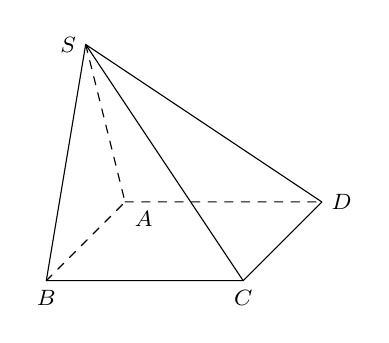
\begin{tikzpicture}[scale=0.5, font=\footnotesize, line join=round, line cap=round, >=stealth]
\draw (1,6)--(0,0)--(5,0)--(7,2)--(1,6)--(5,0);
\draw[dashed] (1,6)--(2,2)--(0,0)(2,2)--(7,2);
\draw (1,6) node[left]{$S$};
\draw (2,2) node[below right]{$A$};
\draw (0,0) node[below]{$B$};
\draw (5,0) node[below]{$C$};
\draw (7,2) node[right]{$D$};
\coordinate(S) at (1,6);
\coordinate(H) at (1,1);
\coordinate(B) at (0,0);
\end{tikzpicture}
}
}
\end{ex}

%%%%%%%%%%%%Câu 18
\begin{ex}%[Thi Thử L1, Sở Bắc Giang, 2023]%[Thành Đức Trung, dự án 12-EX-6]%[2D1B2-1]
Cho hàm số $y=f(x)$ có đạo hàm $f'(x)=x^2(1-x^2)$ với mọi $x\in\mathbb{R}$. Hàm số đã cho nghịch biến trên khoảng nào dưới đây?
\choice
{$(0;+\infty)$}
{$(-1;0)$}
{$(-\infty;0)$}
{\True $(1;+\infty)$}
\loigiai
{Bảng xét dấu đạo hàm của hàm số $y=f(x)$
\begin{center}

\begin{tikzpicture}
\tkzTabInit[lgt=2,espcl=1.5]
{$x$/1, $f'(x)$/1} % cột 1
{$-\infty$,$-1$,$0$,$1$,$+\infty$}
\tkzTabLine{, - , 0 , + , 0 , + , 0, -, } 
\end{tikzpicture}
\end{center}
Dựa vào bảng xét dấu đạo hàm ta thấy hàm số $y=f(x)$ nghịch biến trên khoảng $(1;+\infty)$.
}
\end{ex}

%%%%%%%%%%%%Câu 25
\begin{ex}%[Thi Thử L1, Sở Bắc Giang, 2023]%[Thành Đức Trung, dự án 12-EX-6]%[2D3B3-1]
Diện tích hình phẳng giới hạn bởi đồ thị hàm số $y=x^2+2x$ và trục hoành bằng
\choice
{$\dfrac{4\pi}{3}$}
{\True $\dfrac{4}{3}$}
{$\dfrac{3}{4}$}
{$\dfrac{3\pi}{4}$}
\loigiai
{Xét phương trình hoành độ giao điểm của đồ thị hàm số $y=x^2+2x$ và trục hoành 
$$x^2+2x=0\Leftrightarrow\hoac{&x=-2\\&x=0.}$$
Diện tích hình phẳng giới hạn bởi đồ thị hàm số đã cho với trục hoành bằng
\[S=\displaystyle\int\limits_{-2}^0|x^2+2x|\mathrm{\,d}x=\displaystyle\int\limits_{-2}^0(-x^2-2x)\mathrm{\,d}x=\dfrac{4}{3}.\]
}
\end{ex}

%%%%%%%%%%%%Câu 39
\begin{ex}%[Thi Thử L1, Sở Bắc Giang, 2023]%[Thành Đức Trung, dự án 12-EX-6]%[2H1B3-2]
Cho hình chóp $S \cdot A B C D$ có đáy $A B C D$ là hình chữ nhật với $A B=2 a$, $B C=a \sqrt{3}$. Cạnh bên $S A$ vuông góc với đáy và đường thẳng $S C$ tạo với mặt phẳng $(S A B)$ một góc $30^{\circ}$. Tính thể tích $V$ của khối chóp $S . A B C D$ theo $a$.
\choice
{$V=2 a^3 \sqrt{15}$}
{\True $V=\dfrac{2 a^3 \sqrt{15}}{3}$}
{$V=\dfrac{a^3 \sqrt{3}}{3}$}
{$V=\dfrac{a^3 \sqrt{15}}{3}$}
\loigiai
{
\immini{
Ta có $CB\perp\left(SAB\right)$ nên $B$ là hình chiếu của $C$ lên $\left(SAB\right)$.\\
Suy ra $\left(SC,\left(SAB\right)\right)=\left(SC,SB\right) = \widehat{CSB}$.\\
Xét $\triangle SBC$ vuông tại $B$, ta có $SB = BC\cdot\cot\widehat{CSB} = a\sqrt{3} \cdot\cot30^\circ = 3a$.\\
Xét $\triangle SAB$ vuông tại $A$, ta có $SA = \sqrt{SB^2 - AB^2} = a\sqrt{5}$.\\
Suy ra \[V_{S.ABCD} = \dfrac{1}{3}\cdot S_{ABCD}\cdot SA = \dfrac{2a^3\sqrt{15}}{3}.\]
}{
\begin{tikzpicture}[scale=1, font=\footnotesize, line join=round, line cap=round, >=stealth]
\path
(0,0)coordinate(A)
(-1.5,-1.5)coordinate(B)
(4,0)coordinate(D)
($(B)+(D)-(A)$)coordinate(C)
($(A)+(0,3.5)$)coordinate(S)
;
\draw(B)--(C)--(D) (S)--(B) (S)--(C) (S)--(D);
\draw[dashed](B)--(A)--(D)--(B) (C)--(A)--(S);
\foreach \x/\g in{A/150, B/-90, C/-90, D/0, S/90}
\fill[black](\x)circle(1pt)($(\x)+(\g:2mm)$)node{$\x$};
\tkzMarkRightAngle(S,A,D);\tkzMarkRightAngle(S,B,C);
\end{tikzpicture}
}
}
\end{ex}

%%%%%%%%%%%%Câu 42
\begin{ex}%[Thi Thử L1, Sở Bắc Giang, 2023]%[Thành Đức Trung, dự án 12-EX-6]%[2H3B3-2]
Trong KG $Oxyz$, cho tam giác $ABC$ có $A(- 1; 3; 2) , B(2; 0; 5), C(0; -2;1)$. Viết PTĐT $d$ chứa đường trung tuyến kẻ từ đỉnh $A$ của tam giác $ABC$.
\choice
{$d\colon\dfrac{x-1}{2}=\dfrac{y-3}{-4}=\dfrac{z+2}{1}$}
{\True $d\colon\dfrac{x+1}{2}=\dfrac{y-3}{-4}=\dfrac{z-2}{1}$}
{$d\colon\dfrac{x-1}{2}=\dfrac{y+3}{4}=\dfrac{z+2}{-1}$}
{$d\colon\dfrac{x-2}{1}=\dfrac{y+4}{-1}=\dfrac{z+1}{3}$}
\loigiai{
Gọi $M$ là trung điểm $BC$ suy ra $M(1;- 1; 3)$ và $\overrightarrow{AM}=(2;-4;1)$.\\
Đường trung tuyến $AM$ qua $A$ có véc-tơ chỉ phương $\overrightarrow{AM}$ có phương trình là $d\colon\dfrac{x+1}{2}=\dfrac{y-3}{-4}=\dfrac{z-2}{1}$.
}
\end{ex}

%%%%%%%%%%%%Câu 43
\begin{ex}%[Thi Thử L1, Sở Bắc Giang, 2023]%[Thành Đức Trung, dự án 12-EX-6]%[2H3B2-7]
Trong KG $Oxyz$, cho điểm $A(1;-1;1)$ và đường thẳng $d \colon \heva{&x=t\\&y=-1-2t\\&z=2-2t}, (t\in \mathbb{R})$. Gọi
$(P)$ là mặt phẳng đi qua $A$ và chứa $d$. Lập phương trình mặt cầu $(S)$ có tâm $I(2; 3;-1)$ sao cho $(P)$ tiếp xúc với $(S)$.
\choice
{$(S)\colon(x-2)^2+(y-3)^2+(z+1)^2=16$}
{$(S)\colon(x-2)^2+(y-3)^2+(z+1)^2=9$}
{\True $(S)\colon(x-2)^2+(y-3)^2+(z+1)^2=4$}
{$(S)\colon(x+2)^2+(y+3)^2+(z-1)^2=4$}
\loigiai
{Ta có 
$d$ qua $M(0;- 1; 2)$ và có véc-tơ chỉ phương $\overrightarrow{u}=(1; - 2; - 2)$.\\
Mặt phẳng $(P)$ có véc-tơ pháp tuyến $\overrightarrow{n}=[\overrightarrow{AM},\overrightarrow{u}]=(2;- 1; 2)$.\\
Phương trình mặt phẳng $(P)\colon 2 x - y +2 z -5 = 0$.\\
Bán kính mặt cầu $R= \mathrm{d}(I,(P)) =2$.\\
Vậy phương trình mặt cầu $(S)$ là $(S)\colon(x-2)^2+(y-3)^2+(z+1)^2=4$.
}
\end{ex}

%%%%%%%%%%%%Câu 45
\begin{ex}%[Thi Thử L1, Sở Bắc Giang, 2023]%[Thành Đức Trung, dự án 12-EX-6]%[2D3B2-4]
Cho $F(x)=\dfrac{1}{2x^2}$ là một nguyên hàm của hàm số $\dfrac{f(x)}{x}$ trên $(0;+\infty)$. Tính tích phân $\displaystyle\int\limits_1^2f(2x+1)\mathrm{\,d}x.$
\choice
{$\displaystyle\int\limits_1^2f(2x+1)\mathrm{\,d}x=\dfrac{2}{15}$}
{$\displaystyle\int\limits_1^2f(2x+1)\mathrm{\,d}x=-\dfrac{2}{15}$}
{$\displaystyle\int\limits_1^2f(2x+1)\mathrm{\,d}x=\dfrac{1}{15}$}
{\True $\displaystyle\int\limits_1^2f(2x+1)\mathrm{\,d}x=-\dfrac{1}{15}$}
\loigiai
{Ta có $F'(x)=\dfrac{f(x)}{x}=\left(\dfrac{1}{2x^2}\right)'=-\dfrac{1}{x^3}\Rightarrow f(x)=-\dfrac{1}{x^2}$.\\
Vậy $\displaystyle\int\limits_1^2f(2x+1)\mathrm{\,d}x=-\displaystyle\int\limits_1^2\dfrac{1}{(2x+1)^2}\mathrm{\,d}x=-\dfrac{1}{15}.$
}
\end{ex}

%%%%%%%%%%%%Câu 16
\begin{ex}%[Thi Thử L1, Sở Bắc Giang, 2023]%[Thành Đức Trung, dự án 12-EX-6]%[1D2K5-2]
Xếp ngẫu nhiên 3 quả cầu màu đỏ có kích thước khác nhau và 3 quả cầu màu xanh giống nhau vào một giá chứa đồ nằm ngang có 7 ô trống, mỗi quả cầu được xếp vào một ô. Tính xác suất để 3 quả cầu màu đỏ xếp cạnh nhau và 3 quả cầu màu xanh xếp cạnh nhau.
\choice
{$\dfrac{3}{140}$}
{\True $\dfrac{3}{70}$}
{$\dfrac{3}{160}$}
{$\dfrac{3}{80}$}
\loigiai
{Không gian mẫu là tập các kết quả khi xếp 3 quả cầu màu đỏ có kích thước khác nhau và 3 quả cầu màu xanh giống nhau vào 7 ô trống.\\
Số phần tử không gian mẫu là $n(\Omega)=\dfrac{\mathrm{C}_7^6\cdot 6!}{3!}$.\\
Gọi A là biến cố 3 quả cầu màu đỏ khác nhau xếp cạnh nhau và 3 quả cầu màu xanh giống nhau xếp cạnh nhau.\\
Muốn sắp xếp 3 quả cầu màu đỏ khác nhau và 3 quả cầu xanh giống nhau ta làm theo các giai đoạn như sau:
\begin{itemize}
\item Coi 3 quả cầu màu đỏ khác nhau là 1 quả cầu X: có $3!$ cách.
\item Coi 3 quả cầu màu xanh giống nhau là 1 quả cầu Y: có 1 cách.
\item Sắp xếp 1 quả cầu X và 1 quả cầu Y vào 3 ô trống: có 3! cách.
\end{itemize}
Số phần tử của biến cố A là $n(\text{A})=3!\cdot 1\cdot 3!=36$.\\
Xác suất cần tìm là $\mathrm{P}(\text{A})=\dfrac{n(\text{A})}{n(\Omega)}=\dfrac{3}{70}$.
}
\end{ex}

%%%%%%%%%%%%Câu 36
\begin{ex}%[Thi Thử L1, Sở Bắc Giang, 2023]%[Thành Đức Trung, dự án 12-EX-6]%[2D1K2-2]
Cho hàm số $y=f(x)$, bảng biến thiên của hàm số $f'(x)$ như sau.
\begin{center}

\begin{tikzpicture}[scale = 1, line join=round, line cap=round, >=latex]
\tkzTabInit[lgt=1.2, espcl=2.0, deltacl=0.6]{$x$ /0.6, $f'(x)$ /2.25}{$-\infty$, $-1$, $0$, $1$, $+\infty$}
\tkzTabVar{+/$+\infty$, -/$-3$, +/$2$, -/$-1$, +/$+\infty$}
\end{tikzpicture}
\end{center}
Số điểm cực trị của hàm số $y=f\left(x^2-2 x\right)$ là
\choice
{$9$}
{$5$}
{\True $7$}
{$3$}
\loigiai
{
Ta có $y' = \left(2x-2\right)\cdot f'\left(x^2 - 2x\right) = 0\Leftrightarrow \hoac{&2x-2 = 0\\&f'\left(x^2 - 2x\right) = 0} \Leftrightarrow\hoac{ &x=1\\&\hoac{ &x^2-2x=a\in\left(-\infty;-1\right)&&\qquad(1) \\ &x^2-2x=b\in\left(-1;0\right)&&\qquad(2) \\&x^2-2x=c\in\left(0;1\right)&&\qquad(3)\\&x^2-2x=d\in\left(1;+\infty\right)&&\qquad (4). }}$\\
Xét hàm số $y = x^2 - 2x$ có đồ thị như hình vẽ dưới đây.
\begin{center}
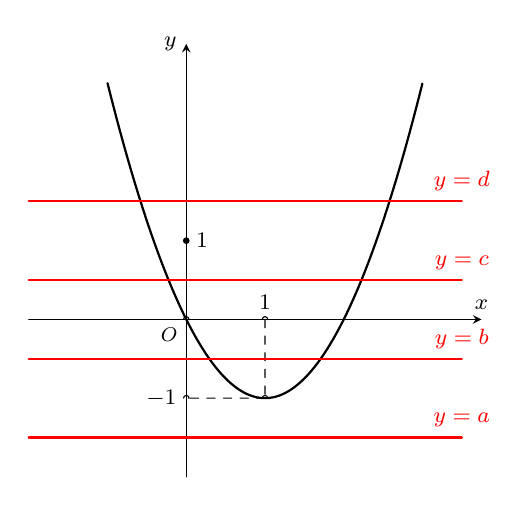
\begin{tikzpicture}[scale = 1, font=\footnotesize, line join=round, line cap=round, >=stealth]
\draw[->] (-2,0) -- (0,0) node[below left, scale = 0.9]{$O$} -- (3.75,0) node[above]{$x$};
\draw[->] (0,-2) -- (0,3.5) node[left]{$ y $};
\draw[color = black, thick] plot[domain=-1:3, samples=100](\x,{(\x)^(2)-2*(\x)});
\draw [dashed] (1,0) circle (1pt) node[above]{$ 1 $} -- (1,-1) circle (1pt) -- (0,-1) circle (1pt) node[left]{$ -1 $} (0,0) circle (1pt);
\draw[fill=black] (0,1) circle (1pt) node[right]{$1$};
\draw[thick,red] (-2,-1.5)--(3.5,-1.5) node[above]{$y=a$};
\draw[thick,red] (-2,-.5)--(3.5,-.5) node[above]{$y=b$};
\draw[thick,red] (-2,.5)--(3.5,.5) node[above]{$y=c$};
\draw[thick,red] (-2,1.5)--(3.5,1.5) node[above]{$y=d$};
\end{tikzpicture}
\end{center}
Dựa vào đồ thị ta thấy phương trình $(1)$ không có nghiệm, phương trình $(2)$, $(3)$ và $(4)$ mỗi phương trình có 2 nghiệm đơn khác $1$.\\
Vậy phương trình $y' = 0$ có tổng cộng $7$ nghiệm đơn, tức là hàm số $y = f\left(x^2-2x\right)$ có $7$ điểm cực trị.
}
\end{ex}

%%%%%%%%%%%%Câu 37
\begin{ex}%[Thi Thử L1, Sở Bắc Giang, 2023]%[Thành Đức Trung, dự án 12-EX-6]%[2H2K2-6]
Cho khối nón tròn xoay đỉnh $S$, đáy là đường tròn tâm $O$, góc ở đỉnh bằng $120^{\circ}$. Mặt phẳng $(Q)$ thay đổi, đi qua $S$ và cắt khối nón theo thiết diện là tam giác $S A B$. Biết rằng giá trị lớn nhất diện tích tam giác $S A B$ là $2 a^2$. Khoảng cách từ $O$ đến mặt phẳng $(Q)$ trong trường hợp diện tích tam giác $S A B$ đạt giá trị lớn nhất là
\choice
{\True $\dfrac{a \sqrt{2}}{2}$}
{$\dfrac{a \sqrt{3}}{2}$}
{$a \sqrt{2}$}
{$\dfrac{a \sqrt{6}}{2}$}
\loigiai
{
\immini{
Xét hình nón $(N)$ có đỉnh $ S $, tâm đáy $ O $, mặt phẳng $\left(Q\right)$ cắt $\left(N\right)$ theo thiết diện là $\triangle SAB$. Ta có
\[S_{\triangle SAB} = \dfrac{1}{2}\cdot SA\cdot SB\cdot\sin\widehat{ASB}\le \dfrac{1}{2}\cdot SA \cdot SB\cdot 1 = \dfrac{l^2}{2}.\]
Suy ra giá trị lớn nhất diện tích $\triangle S A B$ đạt được khi $\triangle SAB$ vuông cân tại $S$. \\
Khi đó ta có $\dfrac{l^2}{2} = 2 a^2 \Leftrightarrow l=2a$.\\
Lại có $AB = SA\cdot\sqrt{2} = 2a\sqrt{2}\Rightarrow SI = \dfrac{1}{2}AB = a\sqrt{2}$.\\
Xét $\triangle SOB$ có $SB = 2a$ và $\widehat{OSB} = 60^\circ$, suy ra $SO = SB\cdot\cos\widehat{OSB} = a$.
}{
\begin{tikzpicture}[scale=0.8, font=\footnotesize, line join=round, line cap=round, >=stealth]
\def \x{3} %bán kính trục lớn elip
\def \y{0.7} %bán kính trục bé elip
\def \h{5.5} %chiều cao hình nón
\coordinate (O) at (0,0);
\coordinate (S) at ($(O)+(0,\h)$);
\coordinate (l) at (180:\x cm and \y cm);
\coordinate (r) at (0:\x cm and \y cm);
\coordinate (A) at (-75:\x cm and \y cm);
\coordinate (B) at (40:\x cm and \y cm);
\coordinate (I) at ($(A)!0.5!(B)$);
\coordinate (H) at ($(S)!3/5!(I)$);
\draw[dashed] (r) arc (0:180:\x cm and \y cm);
\draw (r) arc (0:-180:\x cm and \y cm);
\draw (l)--(S)--(r) (S)--(A);
\draw[dashed] (O)--(A)--(B)--(O)--(I)--(S)--(O)--(H) (S)--(B);
\foreach \diem/\g in {S/90,O/-135,A/-60,B/-75,I/-45,H/45}	\fill (\diem)circle(1.5pt) ($(\diem)+(\g:3mm)$) node{$\diem$};
\end{tikzpicture}
}
\noindent Kẻ $ OI \perp AB \Rightarrow I$ là trung điểm $ AB $.\\
Xét $\triangle SOI$ vuông tại $O$, có $OI = \sqrt{SI^2 - SO^2} = \sqrt{2a^2 - a^2}=a$.\\
Ta có $ \heva{&SO \perp AB\\&OI \perp AB} $ suy ra $ AB\perp (SOI)$.\\
Kẻ $ OH \perp SI \Rightarrow OH \perp (SAB) \Rightarrow  OH=\mathrm{d}(O,(SAB))$.\\
Xét tam giác $ SOI $ vuông tại $ O $, ta có 
\[\dfrac{1}{OH^2} =\dfrac{1}{OS^2}+\dfrac{1}{OI^2} \Leftrightarrow OH = \dfrac{SO\cdot OI}{\sqrt{SO^2 + OI^2}} = \dfrac{a\sqrt{2}}{2}.\]	
}
\end{ex}

%%%%%%%%%%%%Câu 38
\begin{ex}%[Thi Thử L1, Sở Bắc Giang, 2023]%[Thành Đức Trung, dự án 12-EX-6]%[2D4K5-2]
Cho số phức $z$ thỏa mãn điều kiện $\left|z^2+2 z+2\right|=|z+1-i|$. Giá trị lớn nhất của $|z|$ bằng
\choice
{$2 \sqrt{2}-1$}
{$\sqrt{2}-1$}
{\True $\sqrt{2}+1$}
{$\sqrt{2}$}
\loigiai
{
Ta có \[
\begin{aligned}
\left|z^2+2 z+2\right|=\left|z+1-i\right| &\Leftrightarrow \left|\left(z+1-i\right)\left(z+1+i\right)\right| = \left|z+1-i\right|\\
& \Leftrightarrow\left|z+1-i \right|\cdot\left|z+1+i \right| = \left|z+1-i\right|\\
& \Leftrightarrow \heva{&\left|z+1-i\right| = 0\\&\left|z+1+i \right| = 1.}
\end{aligned}
\]
\begin{itemize}
\item Trường hợp 1: $\left|z+1-i \right| = 0 \Leftrightarrow z = -1 + i$. Khi đó $\left|z \right| = \sqrt{2}$.
\item Trường hợp 2: $\left|z+1+i \right| = 1$. Áp dụng bất đẳng thức $\left|z+w \right|\ge \left|\left| z\right|-\left|w \right|\right|$ ta có
\[\left| z+1+i\right|\ge \left|\left|z \right|-\left|1+i \right|\right|  \Leftrightarrow 1\ge \left|\left| z\right| - \sqrt{2}\right| \Leftrightarrow \sqrt{2}-1\le \left| z\right| \le \sqrt{2}+1.\]
\end{itemize}
Vậy giá trị lớn nhất của $|z|$ bằng $\sqrt{2}+1$.
}
\end{ex}

%%%%%%%%%%%%Câu 41
\begin{ex}%[Thi Thử L1, Sở Bắc Giang, 2023]%[Thành Đức Trung, dự án 12-EX-6]%[2H3K1-2]
Cho hình chóp $S.ABCD$ có đáy là hình chữ nhật $ABCD$, $SA \perp(ABCD)$. Biết $SA = AB = a$,
$AD = 2a$. Gọi $G$ là trọng tâm tam giác $SAD$. Khoảng cách từ $G$ đến $(SBD)$ bằng
\choice
{$\dfrac{a}{3}$}
{\True $\dfrac{2a}{9}$}
{$\dfrac{2a}{3}$}
{$\dfrac{a}{6}$}
\loigiai
{\immini{ Chọn hệ trục tọa độ $Oxyz$ trong đó
$$A\equiv O(0;0;0); B(a;0;0); D(0; 2a; 0);S(0; 0; a).$$
Trọng tâm $G$ của tam giác $SAD$ có tọa độ $G\left(0;\dfrac{2a}{3};\dfrac{a}{3}\right)$.\\
Ta có
$\overrightarrow{SB} = (a;0; -a); \overrightarrow{SD} = (0; 2a; -a)$, véc-tơ pháp tuyến
 của mặt phẳng $(SBD)$ là\\ $\overrightarrow{n}=[\overrightarrow{SB}, \overrightarrow{SD}] = (2a^2 ;a^2 ; 2a^2 )=(2;1; 2)$.\\
Phương trình mặt phẳng $(SBD)\colon 2x + y + 2z - 2a = 0$.\\
Vậy khoảng cách từ $G$ đến $(SBD)$ là
$$\mathrm{d}(G,(SBD))=\dfrac{\left|\tfrac{2a}{3}+\tfrac{2a}{3}-2a\right|}{\sqrt{2^2+1^2+2^2}}=\dfrac{2a}{9}.$$
}{	\begin{tikzpicture}[>=stealth,line join=round,line cap=round,font=\footnotesize,scale=1]
\def\ad{4} \def\ab{2} \def\h{3.5}
\def\gocA{-150}
\coordinate[label=below:{$A\equiv O$}] (A) at (0,0);
\coordinate[label=above left:{$B$}] (B) at (\gocA:\ab);
\coordinate[label=above right:{$D$}] (D) at (\ad,0);
\coordinate[label=below:{$C$}] (C) at ($(B)+(\ad,0)$);
\coordinate[label=above left:{$S$}] (S) at (0,\h);
\coordinate[label=below:{$x$}] (x) at (\gocA:\ab + 0.5);
\coordinate[label=right:{$y$}] (y) at ($(D)+(0.5,0)$);
\coordinate[label=above:{$z$}] (z) at ($(S)+(0,0.5)$);
\draw[->] (B)--(x);
\draw[->] (D)--(y);
\draw[->] (S)--(z);
\draw (S)--(B)--(C)--(D)--cycle
(S)--(C);
\draw[dashed] (S)--(A)--(B) (A)--(D)(B)--(D);
\foreach \p in {S,A,B,C,D}
\fill (\p) circle (1.1pt);
\node at (0,1.5) [left]{$a$};
\node at (1.5,0.3) [left]{$2a$};
\node at (-0.8,-0.3) [left]{$a$};
\end{tikzpicture}}
}
\end{ex}

%%%%%%%%%%%%Câu 47
\begin{ex}%[Thi Thử L1, Sở Bắc Giang, 2023]%[Thành Đức Trung, dự án 12-EX-6]%[2D2K6-5]
Số nghiệm nguyên của bất phương trình $\log_2x+\log_3x\geq 1+\log_2x\cdot\log_3x$ là
\choice
{$3$}
{\True $2$}
{Vô số}
{$1$}
\loigiai
{Điều kiện $x > 0$.\\
Bất phương trình 
\begin{align*}
&\log_2x+\log_3x\geq 1+\log_2x\cdot\log_3x\\\Leftrightarrow&(\log_2x-1)(\log_3x-1)\leq 0\\\Leftrightarrow&\hoac{&\heva{&\log_2x-1\leq 0\\&\log_3x-1\geq0}\\&\heva{&\log_2x-1\geq 0\\&\log_3x-1\leq0}}\Leftrightarrow \hoac{&\heva{&x\leq 2\\&x\geq3}\\&\heva{&x\geq 2\\&x\leq3}}\Leftrightarrow 2\leq x \leq 3.
\end{align*}
Vậy bất phương trình có $2$ nghiệm nguyên.
}
\end{ex}

%%%%%%%%%%%%Câu 44
\begin{ex}%[Thi Thử L1, Sở Bắc Giang, 2023]%[Thành Đức Trung, dự án 12-EX-6]%[2H3G3-8]
Trong KG $Oxyz$, cho mặt phẳng $(P)\colon x - 2y + 2z = 0$ và ba điểm
$A (2; 0; 2), B (4; 0; 4), C (5; 2; 4)$. Gọi $M$ là điểm di động trên $(P)$ sao cho có một mặt cầu $(S)$ đi qua $A, B$ và tiếp xúc với $(P)$ tại $M$. Khi đó, độ dài đoạn $CM$ có giá trị nhỏ nhất là
\choice
{$3$}
{$\sqrt{10}$}
{$\sqrt{109}$}
{\True $\sqrt{13}$}
\loigiai
{\immini{Gọi $H$ là hình chiếu của $C$ lên mặt phẳng $(P)$. \\
Một véc-tơ chỉ phương của $CH$ là $\overrightarrow{CH}=\overrightarrow{n}_{P}=(1;-2;2)$. \\
Ta có phương trình $CH\colon \heva{ & x=5+t \\ & y=2-2t \\ & z=4+2t.}$ \\
Vì $H\in CH$ nên $H(5+t;2-2t;4+2t)$. \\
Vì $H\in(P)$ nên $5+t-2(2-2t)+2(4+2t)=0 \Leftrightarrow t=-1$. \\
Suy ra $H(4; 4; 2)$. \\
Đường thẳng $AB\colon\heva{&x=2+t\\&y=0\\&z=2+t.}$ \\
Gọi $K$ là giao điểm của $AB$ và $(P)$. \\
Vì $K\in AB$ nên $K(2+t;0;2+t)$. \\
Vì $K\in(P)$ nên $2+t+2(2+t)=0 \Leftrightarrow t=-2$. \\
Suy ra $K(0;0;0)\equiv O$. \\
Ta có $OM^2=OA\cdot OB=2\sqrt{2}\cdot4\sqrt{2}=16\Rightarrow OM = 4$ \\
và $OH =6$.\\
Ta có $MC = \sqrt{9+MH^2}$. \\
Khi đó $MC_{\min}\Leftrightarrow MH_{\min}\Leftrightarrow MH = OH -OM = 2$.\\
Vậy $CM_{\min} = 13.$}
{\begin{tikzpicture}[line cap=round,line join=round,>=triangle 45,x=1.0cm,y=1.0cm]
\coordinate[label=left:{$A$}] (A) at (-0.32,1.15);
\coordinate[label=above:{$B$}] (B) at (1,3.95);
\coordinate[label=below:{$H$}] (H) at (3.6,0);
\coordinate[label=below:{$O$}] (O) at (-0.9,0);
\coordinate[label=above:{$C$}] (C) at (3.6,3);
\coordinate[label=below:{$M$}] (M) at (1.5,0);
\coordinate[label=below:{}] (O') at (1.5,2);
\draw(-1.,2.)-- (-2.,-1.) (-2.,-1.)-- (5.,-1.) (1,3.95)-- (-0.4,1) (-0.4,1)-- (-0.9,0.) (-0.9,0.)-- (3.6,0.) (3.6,0.)-- (3.6,3);
\draw (1.5,2) circle (2cm);
\foreach \p in {A,B,C,M,O,H,O'}
\fill (\p) circle (1pt);
\end{tikzpicture}
}
}
\end{ex}

%%%%%%%%%%%%Câu 46
\begin{ex}%[Thi Thử L1, Sở Bắc Giang, 2023]%[Thành Đức Trung, dự án 12-EX-6]%[2D2G6-5]
Có tất cả bao nhiêu số nguyên dương $y$ sao cho ứng với mỗi số $y$ đó, bất phương trình $\dfrac{x^3-4x^2+x-4}{3^x-y} < 0$ có nghiệm nguyên $x$ và số nghiệm nguyên $x$ không vượt quá $6.$
\choice
{$176903$}
{\True $176930$}
{$176910$}
{$176923$}
\loigiai
{Điều kiện $ x, y \in \mathbb{Z}, y > 0$.\\
Ta có $\dfrac{x^3-4x^2+x-4}{3^x-y} < 0\Leftrightarrow \dfrac{(x-4)(x^2+1)}{3^x-y}<0\Leftrightarrow \dfrac{x-4}{3^x-y}<0\Leftrightarrow (x-4)(3^x-y)<0.$ \quad $(1)$.\\ 
+ TH1: Nếu $\log_3 y > 4 \Leftrightarrow y > 81$ thì bất phương trình $(1) \Leftrightarrow 4 < x < \log_3 y$.\\
Để bất phương trình có nghiệm nguyên $x$ và số nghiệm nguyên $x$ không vượt quá $6$ thì \\
$\heva{&\log_3y\leq 11\\&\log_3y>5}\Leftrightarrow \heva{&y\leq 177147\\&y>234}\Leftrightarrow 243<y\leq 177147$ do đó
có $176904$ số nguyên $y$.\\
+ TH2: Nếu $\log_3 y < 4 \Leftrightarrow y < 81$ thì bất phương trình $(1)\Leftrightarrow \log_3 y < x < 4$.\\
Để bất phương trình có nghiệm nguyên $x$ và số nghiệm nguyên $x$ không vượt quá $6$ thì \\
$\heva{&\log_3y\geq -3\\&\log_3y<3}\Leftrightarrow \dfrac{1}{27}\leq y < 27 $ do đó có $26$ số nguyên $y$.\\
Vậy ta có $176904 + 26 = 176930$ số nguyên $y$ cần tìm.
}
\end{ex}

%%%%%%%%%%%%Câu 48
\begin{ex}%[Thi Thử L1, Sở Bắc Giang, 2023]%[Thành Đức Trung, dự án 12-EX-6]%[2D1G1-3]
Cho hàm số $y=\left|12x^5-(15m+30)x^4+20x^3-30(m^2-4m+3)x^2+120(m^2+1)x+2023+m\right|$.
Có tất cả bao nhiêu giá trị nguyên của tham số $m$ để hàm số đồng biến trên khoảng $(1;3)$?
\choice
{$11$}
{$10$}
{\True $2$}
{$1$}
\loigiai
{Đặt $f(x)=12x^5-(15m+30)x^4+20x^3-30(m^2-4m+3)x^2+120(m^2+1)x+2023+m$.\\
Ta có $f'(x)=60x^4-60(m+2)x^3+60x^2-60(m^2-4m+3)x+120(m^2+1)$,\\
suy ra $f'(x)=0\Leftrightarrow\hoac{&x=2\\&x^3-mx^2+(-2m+1)x-m^2-1=0. \quad (1)}$ \\
Hàm số $y = |f(x)|$ đồng biến trên $(1;3)$ suy ra $y =f(x)$ đồng biến trên $(1;3)$ hoặc nghịch biến trên khoảng $(1;3)$.\\
Do đó $x=2$ không là điểm cực trị của hàm số $f(x)$. \\
Giả sử $x=2$ là không nghiệm của phương trình $(1)$.\\
Khi đó $f'(x)=0$ nhận $x=2$ là nghiệm đơn, do đó $x=2$ là điểm cực trị của $f'(x)$, dẫn tới vô lí. \\
Suy ra $x=2$ là nghiệm của phương trình $(1)$. \\
Điều kiện cần để $x = 2$ là nghiệm của phương trình $(1)$\\
\[8-4m-4m+2-m^2-1=0\Leftrightarrow-m^2-8m+9=0\Leftrightarrow\hoac{&m=1\\&m=-9.}\]
Điều kiện đủ\\
Với $m=1$, khi đó $\heva{&f'(x)=60(x-2)^2(x^2+x+1)\geq 0,\, \forall x \in (1;3)\\&f(1)=2251>0}$ suy ra hàm số $y = |f(x)|$ đồng biến trên $(1;3)$.\\
Với $m =-9$, khi đó $\heva{&f'(x)=60(x-2)^2(x^2+11x+41)\geq 0,\, \forall x \in (1;3)\\&f(1)=8391>0}$ suy ra hàm số $y = |f(x)|$ đồng biến trên $(1;3)$.\\
Vây $m = 1; m =-9$ nên có $2$ giá trị nguyên của $m$ thoả mãn.
}
\end{ex}

%%%%%%%%%%%%Câu 49
\begin{ex}%[Thi Thử L1, Sở Bắc Giang, 2023]%[Thành Đức Trung, dự án 12-EX-6]%[2D3G3-1]
Trong mặt phẳng tọa độ $Oxy$, cho parabol $(P)\colon y =x^2$ và hai điểm $A, B$ thuộc $(P)$ sao cho
$AB= 2$. Diện tích hình phẳng giới hạn bởi $(P)$ và đường thẳng $AB$ đạt giá trị lớn nhất bằng
\choice
{$\dfrac{3}{2}$}
{$\dfrac{3}{4}$}
{$\dfrac{2}{3}$}
{\True $\dfrac{4}{3}$}
\loigiai
{Gọi $A(a;a^2), B(b;b^2)$ với $a<b$. Ta có $AB=2\Leftrightarrow (b-a)^2+(b^2-a^2)^2=4$.\\
PTĐT $AB\colon\dfrac{x-a}{b-a}=\dfrac{y-a^2}{b^2-a^2}\Leftrightarrow\dfrac{x-a}{1}=\dfrac{y-a^2}{b+a}\Leftrightarrow y = (a+b)x-ab.$\\
Diện tích hình phẳng giới hạn bởi $(P)$ và đường thẳng $AB$ là
$$S= \displaystyle\int\limits_a^b |(a+b)x-ab-x^2|\mathrm{\,d}x = \displaystyle\int\limits_a^b |(x-a)(b-x)|\mathrm{\,d}x.$$
Khi $a\leq x \leq b$ thì $(x-a)(b-x)\geq 0$ nên $S= \displaystyle\int\limits_a^b |(x-a)(b-x)|\mathrm{\,d}x$. \\
Đặt $t = x-a\Rightarrow \mathrm{\,d}t=\mathrm{\,d}x$, đổi cận $x=a\Rightarrow t=0; x=b \Rightarrow t = b-a$.\\
Do đó $S= \displaystyle\int\limits_0^{b-a} \left(t(b-a-t)\right)\mathrm{\,d}t=\dfrac{(b-a)^3}{6}.$\\
Ta có $(b-a)^2+(b^2-a^2)^2=4\Leftrightarrow(b-a)^2(1+(b+a)^2)=4\Leftrightarrow(b-a)^2=\dfrac{4}{1+(b+a)^2}\leq 4$.\\
Suy ra $b-a \leq 2 \Rightarrow S = \dfrac{(b-a)^3}{6}\leq \dfrac{2^3}{6}=\dfrac{4}{3}.$\\
Dấu \lq\lq =\rq\rq\, xảy ra $\Leftrightarrow\heva{&a+b=0\\&b-a=2}\Leftrightarrow \heva{&a=-1\\&b=1.}$
}
\end{ex}

%%%%%%%%%%%%Câu 50
\begin{ex}%[Thi Thử L1, Sở Bắc Giang, 2023]%[Thành Đức Trung, dự án 12-EX-6]%[2D4G4-2]
Cho phương trình $z^2-2(m+1)z+6m-2= 0$ ($m$ tham số thực). Hỏi
có tất cả bao nhiêu giá trị nguyên của $m$ để phương trình đã cho có hai nghiệm phân biệt $z_1, z_2$ thỏa mãn $|z_1|=|z_2|$?
\choice
{$0$}
{$1$}
{Vô số}
{\True $2$}
\loigiai
{Xét $z^2-2(m+1)z+6m-2= 0\quad (1)$, ta có $\Delta' = m^2 -4m +3=(m - 1)(m - 3)$.\\
+) TH1: $\Delta' > 0 \Leftrightarrow (m - 1)(m - 3) > 0\Leftrightarrow \hoac{&m>3\\&m<1.}$\\
Khi đó phương trình $(1)$ có hai nghiệm thực phân biệt $z_1; z_2$.\\
Vậy $|z_1|=|z_2| \Leftrightarrow z_1^2=z_2^2 \Leftrightarrow (z_1 - z_2)(z_1 +z_2) = 0$.\\
Do $z_1 ; z_2$ là hai nghiệm phân biệt nên suy ra $z_1+ z_2 =0$.\\
Theo Vi-ét $z_1 + z_2 = 0 \Leftrightarrow 2(m + 1) = 0 \Leftrightarrow m =-1$ (thỏa mãn).\\
+) TH2: $\Delta' < 0 \Leftrightarrow (m - 1)(m - 3) < 0\Leftrightarrow 1 < m < 3\Rightarrow m = 2.$\\
Thì phương trình $(1)$ có hai nghiệm phức phân biệt $z_1 ; z_2\Rightarrow z_1=\overline{z}_2\Rightarrow |z_1| = |z_2|$.\\
Vậy tất cả có $2$ giá trị của $m$ thỏa mãn đề bài là $-1; 2$.
}
\end{ex}

\Closesolutionfile{ans}
\begin{indapan}{10}
{ans/ans-2-TT-4-SoBacGiang-23-L1}
\end{indapan}